\documentclass[
]{beamer}
\usepackage[czech]{babel}
\usepackage[utf8]{inputenc}
\usepackage[T1]{fontenc}
\usepackage{booktabs}

\usetheme[
  workplace=fi,
]{MU}
\begin{document}

\title[Obhajoba diplomové práce]{Autentizační a autorizační infrastruktura pro videokonferenční prostředí}
\subtitle[Short Presentation Subtitle]{Obhajoba diplomové práce}
\author[L.\,Kotol]{Bc. Lukáš Kotol \\ 433265@mail.muni.cz}
\institute[FI MU]{Fakulta informatiky, Masarykova Univerzita}
\date{18. června 2019}
\subject{Presentation Subject}
\keywords{the, presentation, keywords}

\begin{frame}[plain]
\maketitle
\end{frame}

\section[Zadání]{Zadání}

\begin{frame}{Rezervační služba Meetings}

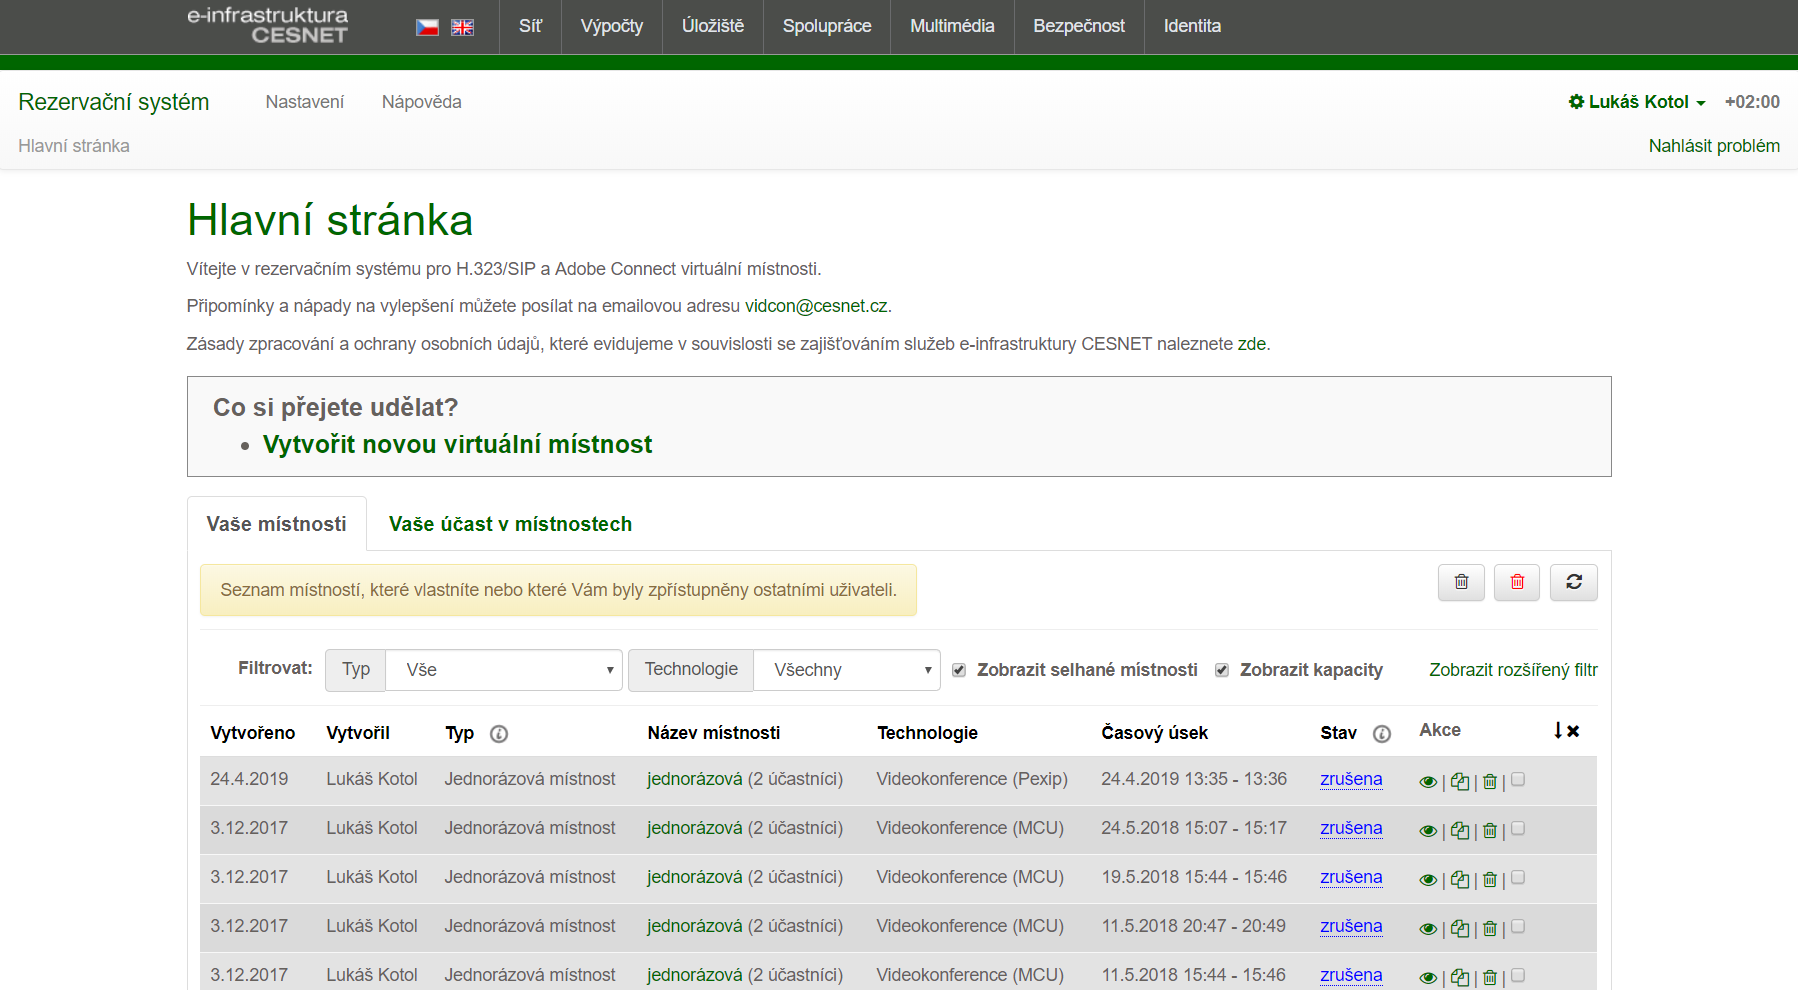
\includegraphics[width=\textwidth]{pics/rezervacni_system}
\end{frame}

\begin{frame}{Webkonferenční služba realizovaná technologií Adobe Connect}

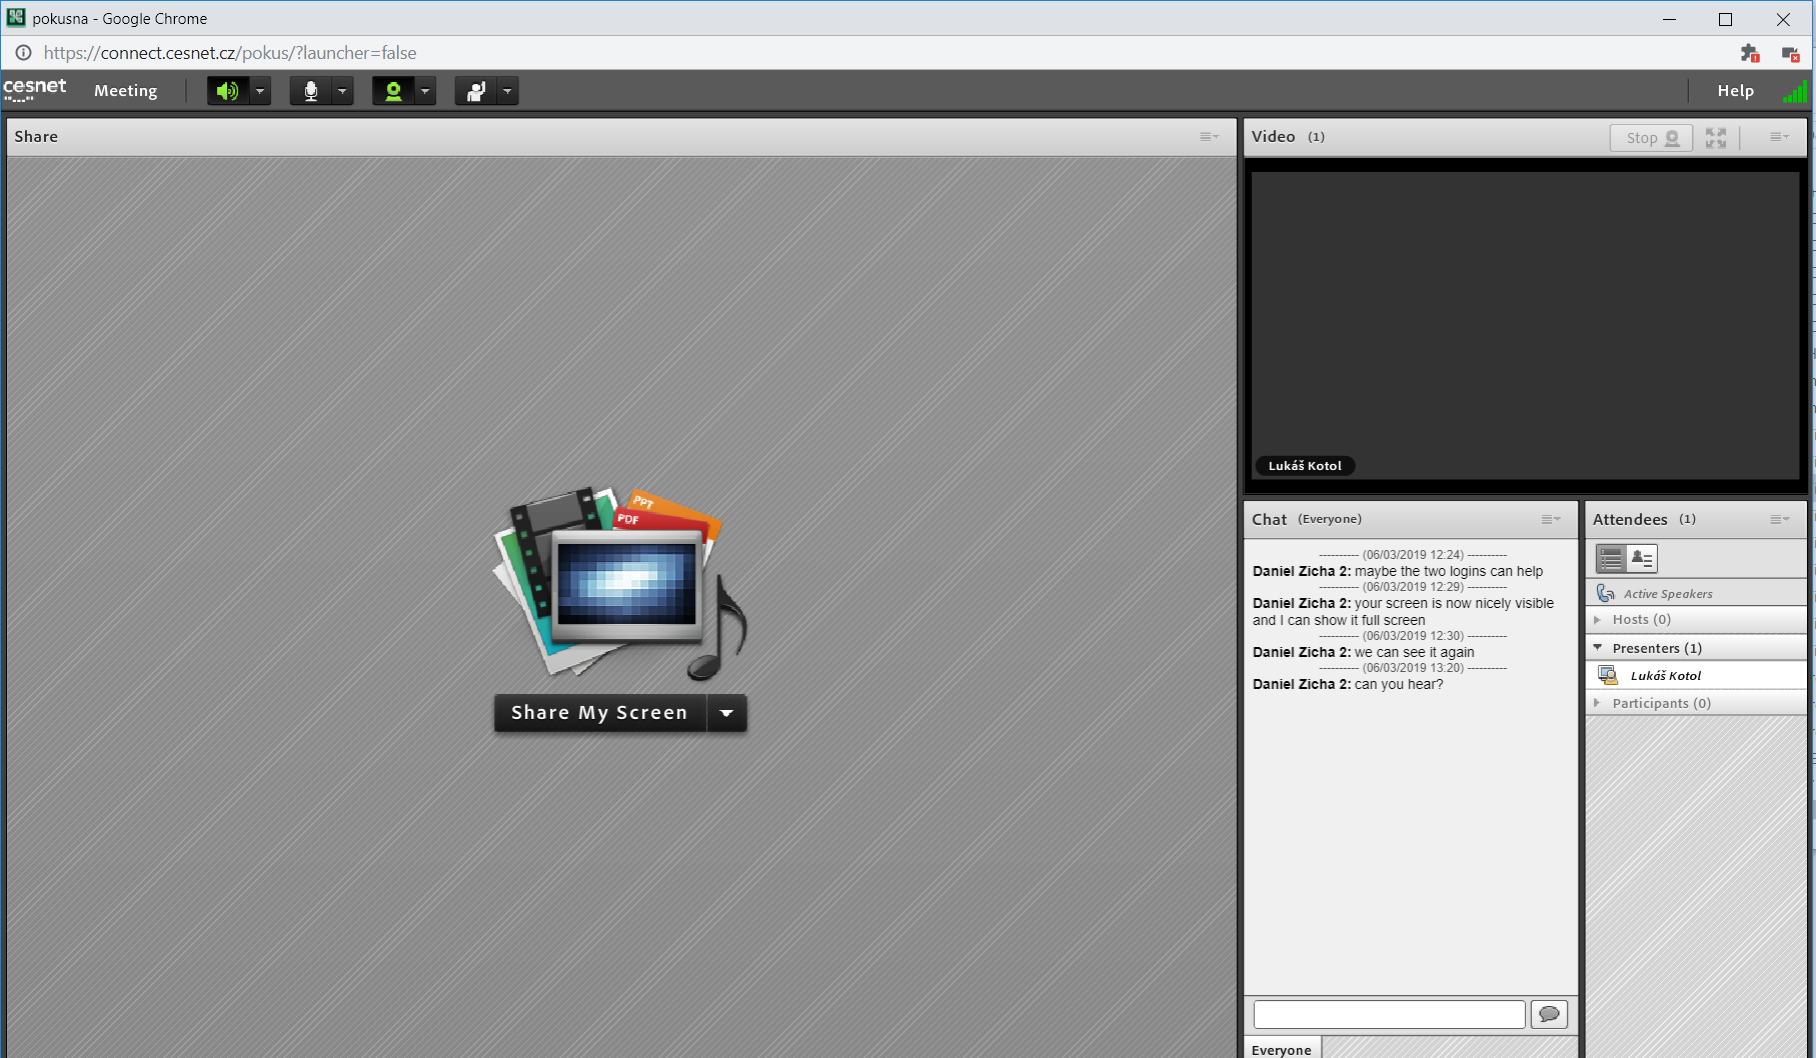
\includegraphics[width=\textwidth]{pics/adobe_connect.PNG}
\end{frame}

\begin{frame}{Schéma komunikace při zpracování autentizačního požadavku ve stávající infrastruktuře}

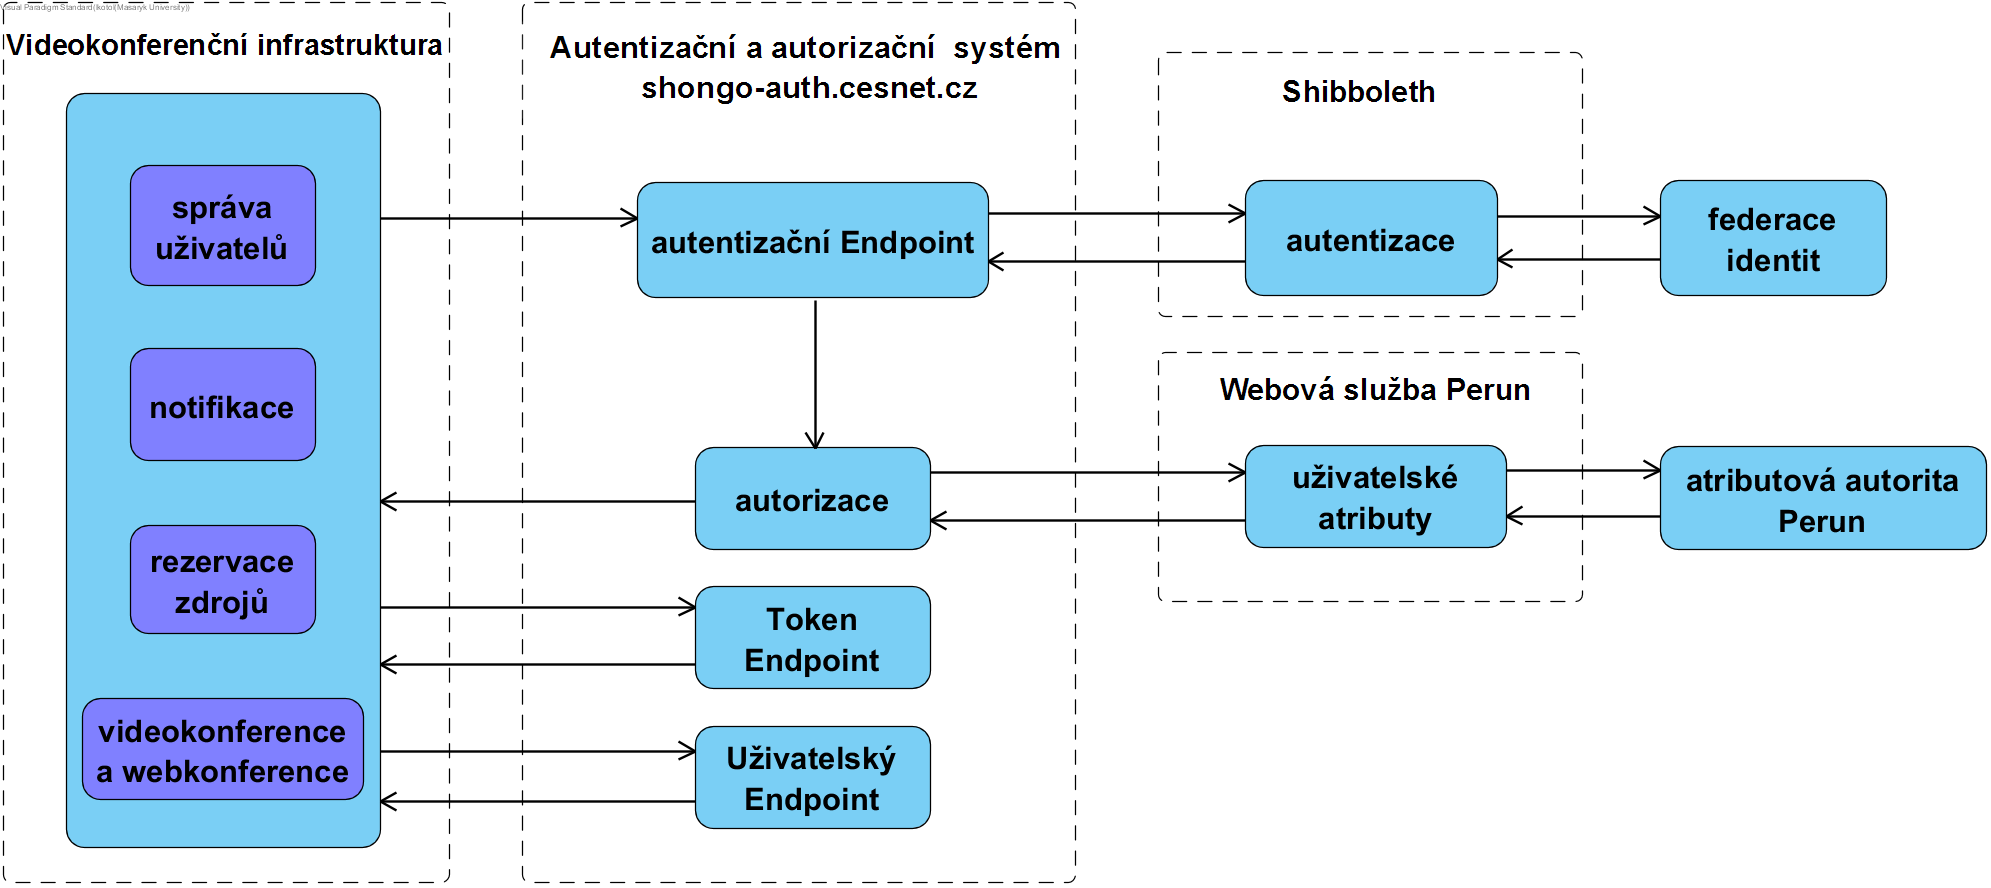
\includegraphics[width=\textwidth]{pics/meetings-old.png}
\end{frame}

\begin{frame}{Schéma komunikace při zpracování autentizačního požadavku ve stávající infrastruktuře}

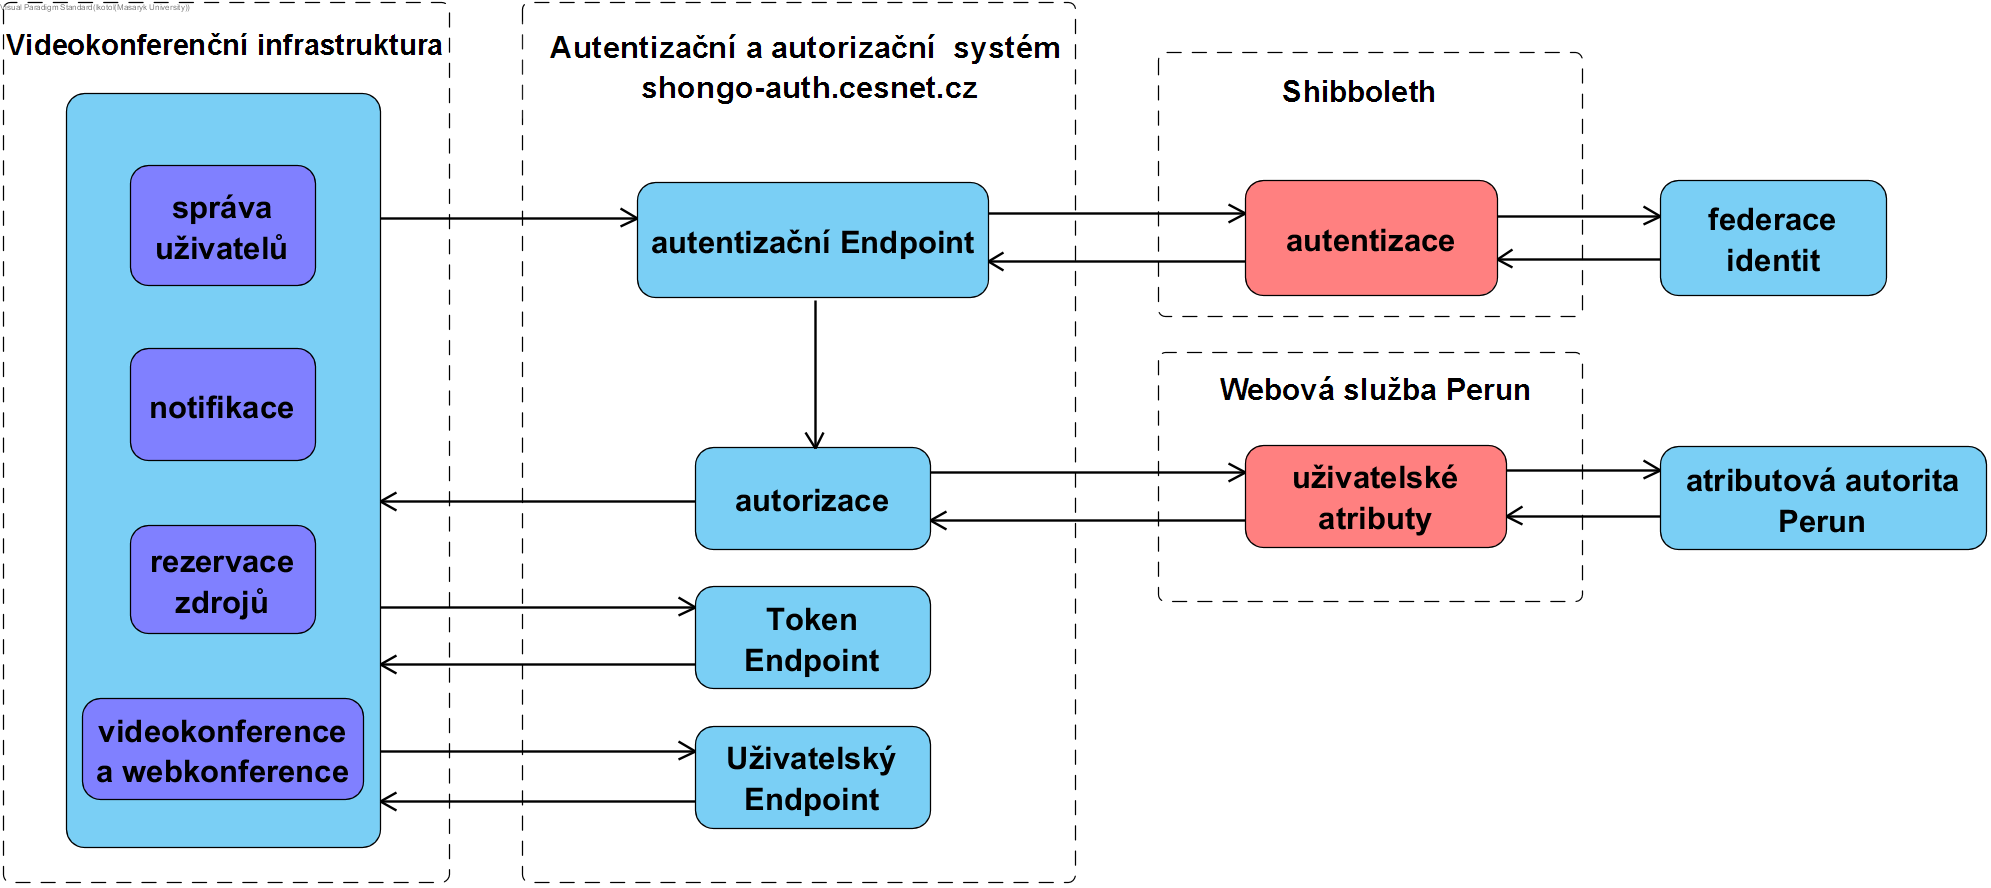
\includegraphics[width=\textwidth]{pics/meetings-old-crash.png}
\end{frame}

\begin{frame}{Schéma komunikace při zpracování autentizačního požadavku}

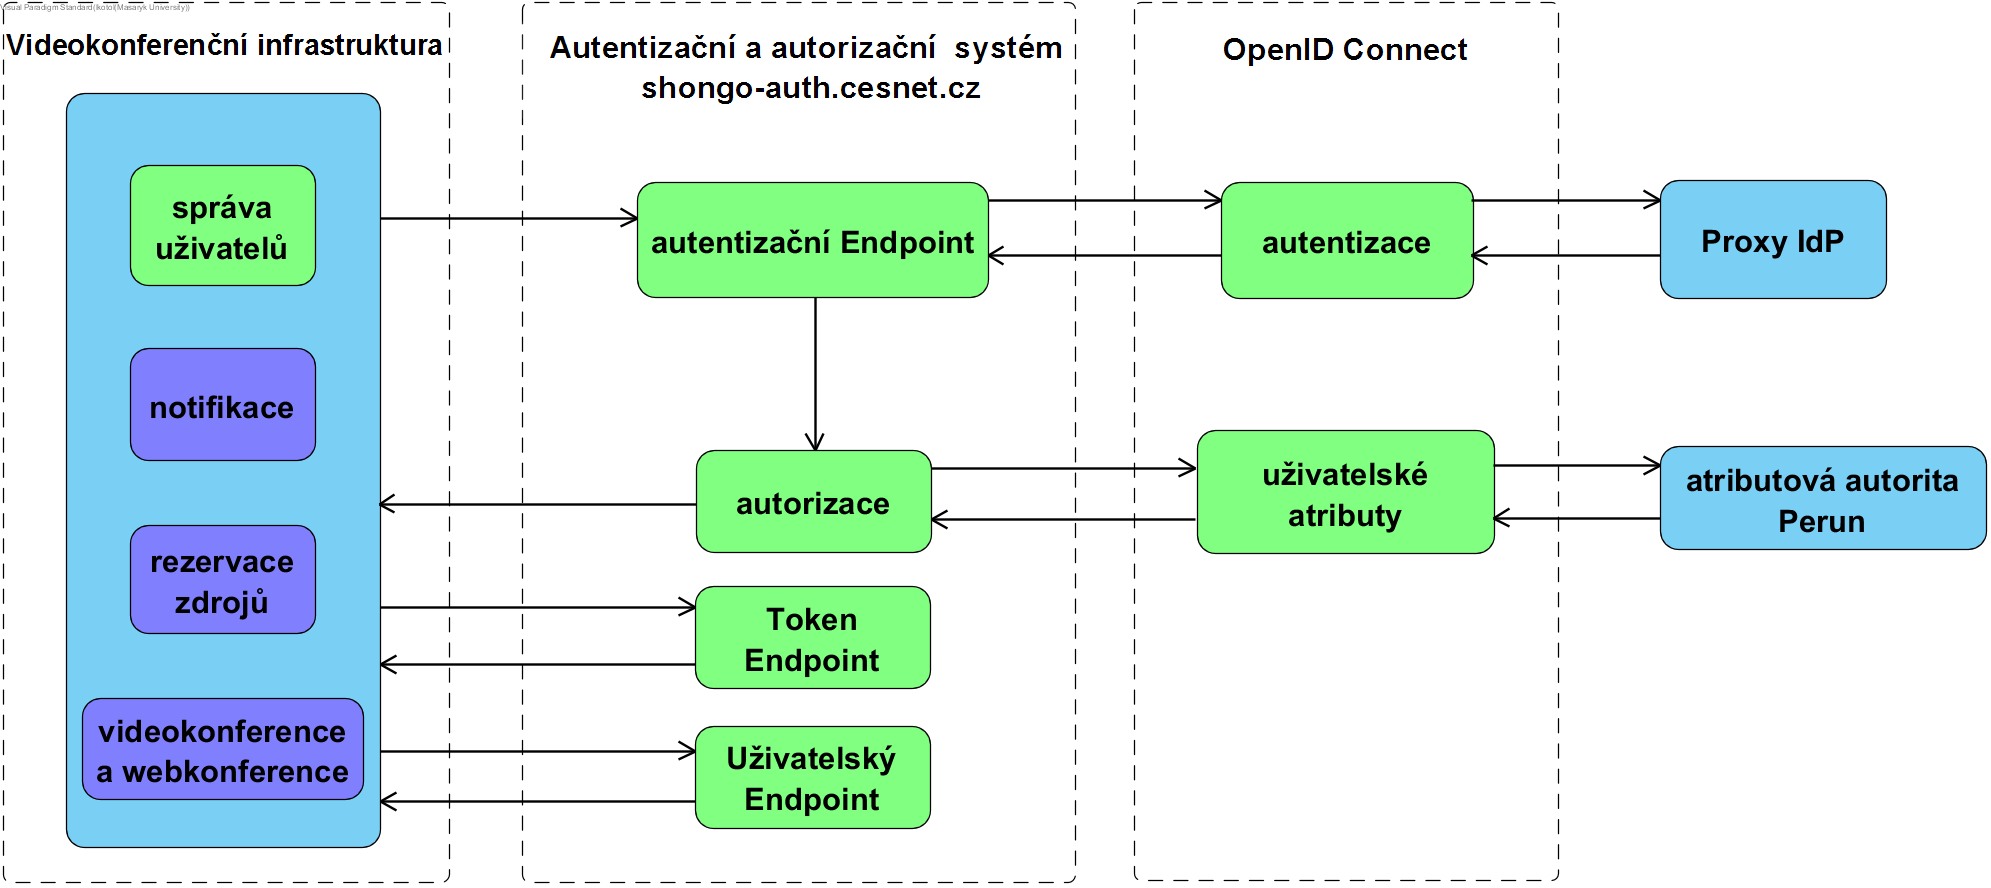
\includegraphics[width=\textwidth]{pics/oidc-new.png}
\end{frame}

\begin{frame}{Návrh řešení}
Nová autentizační a autorizační infrastruktura bude
\begin{itemize}
  \item integrována do \structure{Proxy IdP v infrastruktuře CESNETu},
  \item založena na technologii \structure{OpenID Connect}, 
  \item navazovat na stávající.
\end{itemize}
\end{frame}

\section[Proxy Idp]{Proxy Idp}
\begin{frame}{Proxy IdP infrastruktura}
\begin{itemize}
    \item sdružuje služby a poskytovatele identit,
    \item zajišťuje bezpečný přístup ke službám \structure{CESNET eInfrastruktury} a garantuje dostupnost uživatelských atributů,
    \item umožňuje delegaci procesu autentizace a autorizace.

\end{itemize}
\end{frame}

\section[OpenID Connect]{OpenID Connect}

\begin{frame}{OpenID Connect}
\framesubtitle{Představení protokolu}
Protokol, umožňující aplikaci verifikovat identitu uživatele na základě autentizace provedené autorizačním serverem.
\\
\medskip
Klíčové vlastnosti:
\begin{itemize}
  \item autentizační vrstva nad protokolem \structure{OAuth},
  \item definuje způsob získávání informací o přihlášeném uživateli,
  \item specifikuje koncové body, tzv. \structure{Endpointy}.
\end{itemize}
\end{frame}

\begin{frame}{OpenID Connect}
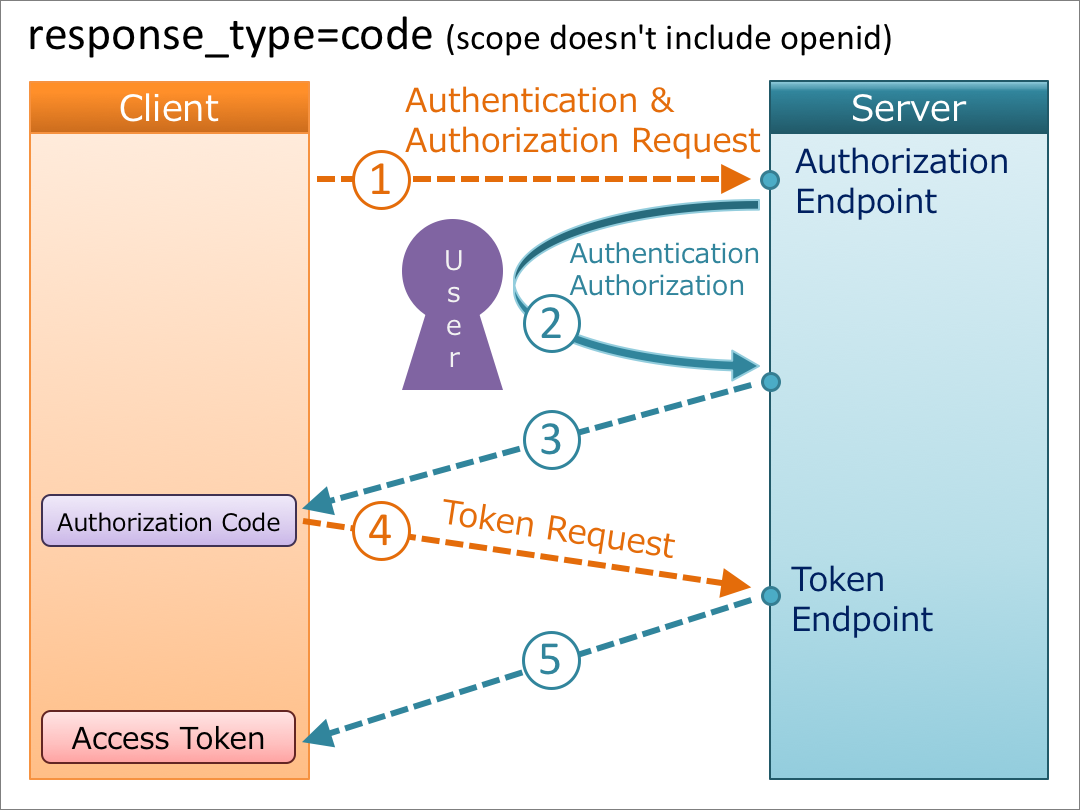
\includegraphics[width=300px,height=200px]{pics/authorization_code_access.png} \\
\begin{tiny}
(https://medium.com/@darutk/diagrams-of-all-the-openid-connect-flows-6968e3990660)
\end{tiny}
\end{frame}

\begin{frame}{OpenID Connect}
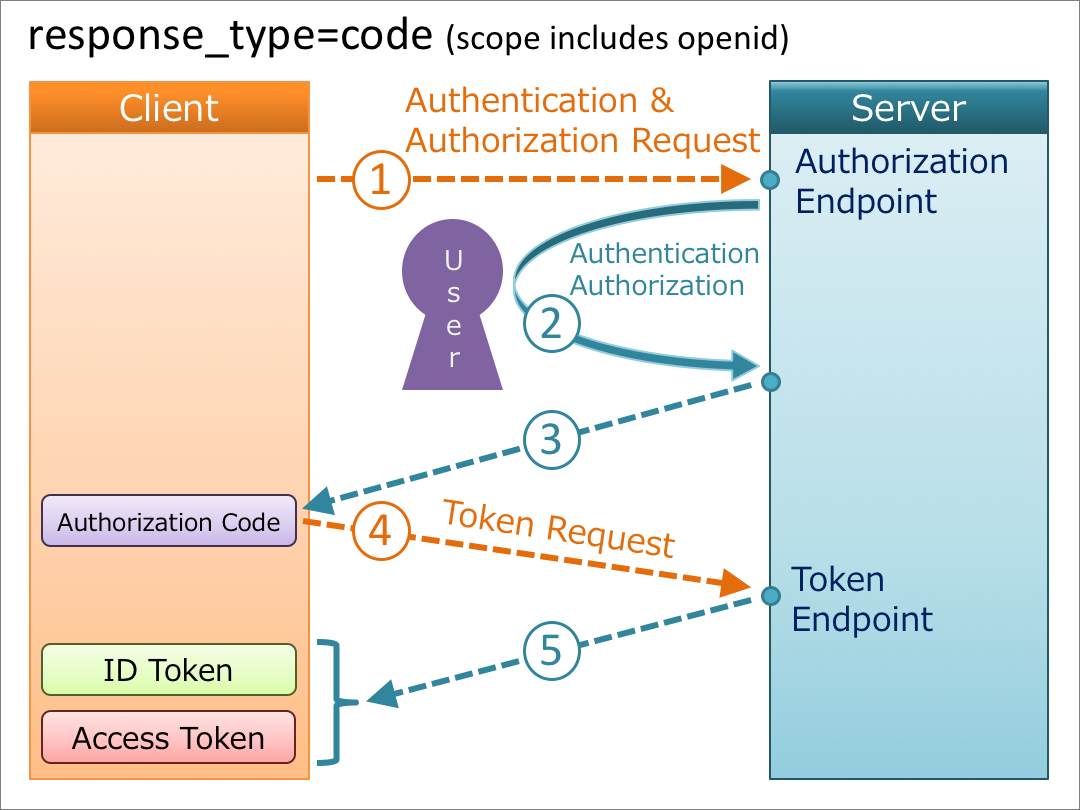
\includegraphics[width=300px,height=200px]{pics/authorization_code_both.png} \\
\begin{tiny}
(https://medium.com/@darutk/diagrams-of-all-the-openid-connect-flows-6968e3990660)
\end{tiny}
\end{frame}

\begin{frame}{OpenID Connect}
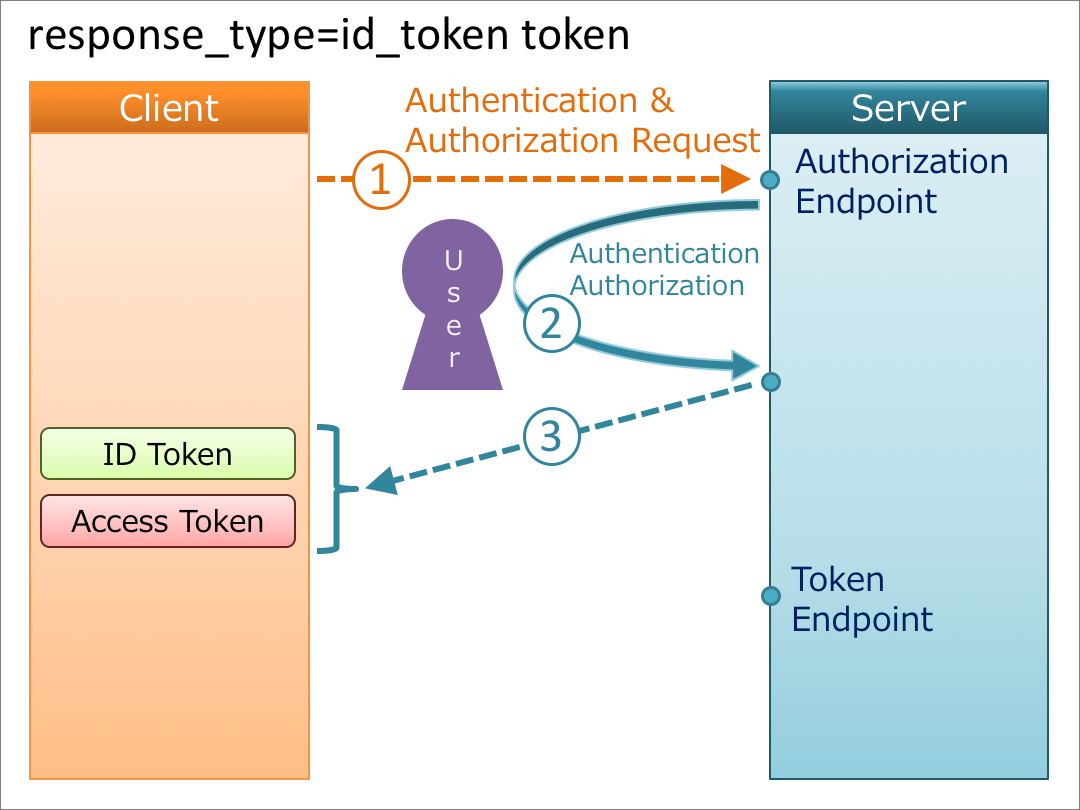
\includegraphics[width=300px,height=200px]{pics/both.png} \\

\begin{tiny}
(https://medium.com/@darutk/diagrams-of-all-the-openid-connect-flows-6968e3990660)
\end{tiny}
\end{frame}


\section[Implementace autentizační a autorizační infrastruktury]{Implementace autentizační a autorizační infrastruktury}

\begin{frame}{Vypracování diplomové práce}
\framesubtitle{Implementace autentizačního a autorizačního procesu}

Na základě návrhu jsem implementoval
\begin{itemize}
     \item delegování autentizace na autentizační server OpenID Connect,
    \item  získání a zpracovaní uživatelských atributů po autentizaci,
    \item  autorizační logiku.
\end{itemize}

\end{frame}

\begin{frame}{Vypracování diplomové práce}
\framesubtitle{Autentizační vrstva služby Adobe Connect}
Navrhl a implementoval jsem
\begin{itemize}
    \item přemapování uživatelských atributů,
    \item logiku vytváření nových uživatelů ve službě Adobe Connect.
\end{itemize}
\end{frame}


\begin{frame}{Vypracování diplomové práce}
\framesubtitle{Reimplementace správy uživatelů v systému Meetings}

Uživatelské údaje se využívaly při
\begin{itemize}
    \item rezervaci požadavků,
    \item notifikaci,
    \item přidávání dalších uživatelů do místnosti. 
\end{itemize}
\end{frame}


\begin{frame}{Schéma komunikace při zpracování autentizačního požadavku}

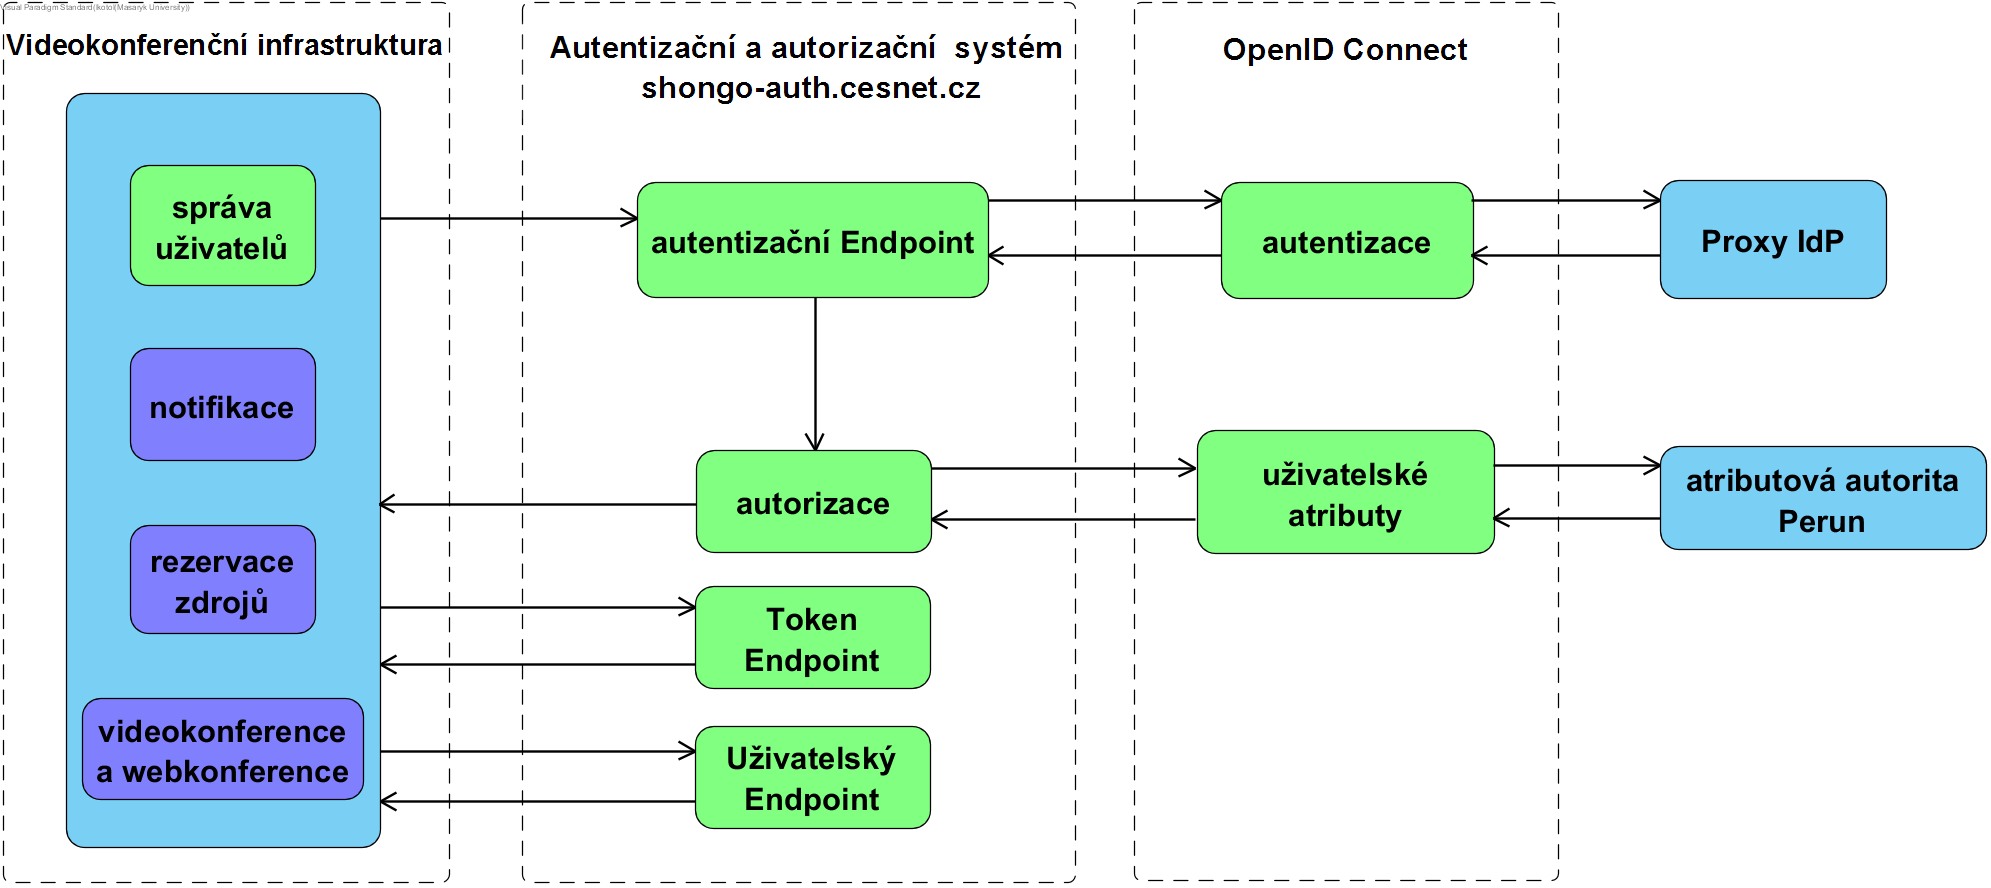
\includegraphics[width=\textwidth]{pics/oidc-new.png}
\end{frame}


\begingroup
\setbeamercolor{background canvas}{bg=mubeamer@base}
\begin{frame}[plain]
\vfill
\centering

\includegraphics[width=\textwidth]{institution}
\vfill
\end{frame}
\endgroup

\end{document}
